\documentclass[]{article}
\usepackage{lmodern}
\usepackage{fancyhdr}
\usepackage{graphicx}
\pagestyle{fancy}
\rhead{Sprawozdanie z projektu w Javie: jaguar}
\usepackage{amssymb,amsmath}
\usepackage[utf8]{inputenc}
\usepackage[english]{babel}
\usepackage{lastpage}
\usepackage{amsmath,amscd}
\usepackage[all,cmtip]{xy}
\usepackage{ifxetex,ifluatex}
\usepackage{fixltx2e} % provides \textsubscript
\ifnum 0\ifxetex 1\fi\ifluatex 1\fi=0 % if pdftex
  \usepackage[T1]{fontenc}
  \usepackage[utf8]{inputenc}
\else % if luatex or xelatex
  \ifxetex
    \usepackage{mathspec}
  \else
    \usepackage{fontspec}
  \fi
  \defaultfontfeatures{Ligatures=TeX,Scale=MatchLowercase}
\fi
% use upquote if available, for straight quotes in verbatim environments
\IfFileExists{upquote.sty}{\usepackage{upquote}}{}
% use microtype if available
\IfFileExists{microtype.sty}{%
\usepackage[]{microtype}
\UseMicrotypeSet[protrusion]{basicmath} % disable protrusion for tt fonts
}{}
\PassOptionsToPackage{hyphens}{url} % url is loaded by hyperref
\usepackage[unicode=true]{hyperref}
\hypersetup{
            pdftitle={Sprawozdanie z projektu w Javie: jaguar},
            pdfauthor={Kuźmicki Maciej, Skiba Szymon},
            pdfborder={0 0 0},
            breaklinks=true}
\urlstyle{same}  % don't use monospace font for urls
\usepackage{multicol}
\IfFileExists{parskip.sty}{%
\usepackage{parskip}
}{% else
\setlength{\parindent}{0pt}
\setlength{\parskip}{6pt plus 2pt minus 1pt}
}
\setlength{\emergencystretch}{3em}  % prevent overfull lines
\providecommand{\tightlist}{%
  \setlength{\itemsep}{0pt}\setlength{\parskip}{0pt}}
\setcounter{secnumdepth}{0}
% Redefines (sub)paragraphs to behave more like sections
\ifx\paragraph\undefined\else
\let\oldparagraph\paragraph
\renewcommand{\paragraph}[1]{\oldparagraph{#1}\mbox{}}
\fi
\ifx\subparagraph\undefined\else
\let\oldsubparagraph\subparagraph
\renewcommand{\subparagraph}[1]{\oldsubparagraph{#1}\mbox{}}
\fi
% set default figure placement to htbp
\makeatletter
\def\fps@figure{htbp}
\makeatother
\title{Sprawozdanie z projektu w Javie: \texttt{jaguar}}
\author{Kuźmicki Maciej, Skiba Szymon}
\date{08.06.2022}
\begin{document}
\maketitle
\thispagestyle{fancy}
\section{Informacje ogólne}\label{header-n231}
\cfoot{Page \thepage \hspace{1pt} of \pageref{LastPage}}
Celem projektu było napisanie programu, który wykonywałby operacje na grafach. Do jego zadań należy generowanie grafu na trzy różne sposoby, sprawdzanie spójności oraz wyznaczanie najkrótszej ścieżki pomiędzy dwoma dowolnymi wierzchołkami. Program napisany został w języku \texttt{Java SE 8} w środowisku programistycznym \texttt{IntelliJ IDEA} z wykorzystaniem pakietu \texttt{Java FX} do utworzenia interfejsu graficznego oraz oprogramowania \texttt{JUnit} do napisania testów jednostkowych. Całość współpracowała ze sobą dzięki oprogramowaniu \texttt{Maven}, które służy do zachowania przenośności kodu.


\section{Zmiany powstałe w trakcie implementacji}\label{header-n233}
 Podczas implementacji zostało wprowadzonych sporo zmian, które zostaną przedstawione poniżej z podziałem na poszczególne klasy (metody w modułach, które pozostały bez zmian zostaną pominięte, odnaleźć je można w specyfikacji implementacyjnej):
\begin{itemize}
\item
\texttt{Main.java} - funkcjonalność tej klasy została ograniczona jedynie do uruchomienia samego programu;
\item
\texttt{BFS.java} - nazwa klasy została zmieniona z Bfs na BFS, tak samo jak nazwa konstruktora, reszta pozostała bez zmian;
\item
\texttt{Vertex.java} - klasa ta została dodana dla lepszego zarządzania grafem, przechowuje informacje wierzchołkach w grafie: ich pozycje(nr kolumny i wiersza), numer wierzchołka oraz liste sąsiadów (Neighbor) czyli krawędzi wychodzących z tego wierzchołka. Metody tej klasy to settery, gettery i konstruktor parametryczny który przyjmuje nr kolumny i wiersza oraz numer wierzchołka;
\item
\texttt{Neighbor.java} - klasa ta została przerobiona dla lepszego zarządzania grafem, przechowuje informacje o "krawędzi" w grafie, danemu wierzchołkowi (obiektowi klasy Vertex) przypisuje się liste obiektów klasy Neighbor które mają w sobie informacje o wadze, drugim wierzchołku krawędzi oraz kolorze krawędzi zgodznym z skalą;
\item
\texttt{Graf.java} - klasa grafu korzysta w ostatecznej wersji z obiektów klas Vertex i Neighbour dla lepszego zarządzania strukturą grafu. Ponadto wszystkie nazwy tej klasy rozpoczynały się z małej litery, w specyfikacji implementacyjnej znajdziemy błędne nazwy rozpoczynające się wielkimi literami, co jest błędem w konwencji nazewnictwa w tym języku i to zostało zmienione, dodatkowo zostały dodane nowe metody, a niektóre zostały usunięte lub zmienione:
\begin{itemize}
\item
\texttt{showNeighbors()} - metoda ta jest odpowiedzialna za wypisanie do String'a wszystkich sąsiadów wszystkich wierzchołków, używana do testowania wczytywania grafu z pliku;
\item
\texttt{addEdge()} - metoda ta jest odpowiedzialna za dodanie krawędzi( instancji klasy Neighbor) do "listy sąsiadów" danego wierzchołk;
\item
\texttt{addVertex()} - metoda ta jest odpowiedzialna za dodanie wierzchołka(instancji klasy Vertex) do listy wierzchołków;
\item
\texttt{readFromFile()} - metoda ta niezmieniła swojej funkcjonalności jednak została przerobiona na statyczną;
\end{itemize}
\item
\texttt{Controller.java} - klasa ta obsługuje wszystkimi zdarzeniami, które umożliwia graficzny interfejs użytkownika, zawiera metody obsługujące przyciski, rysowanie grafu, rysowanie ścieżek oraz klasę wewnętrzną Path która wykorzystywana jest do tworzenia ścieżek oraz ich rysowania wykorzystując wynik algorytmu dijkstry który zwraca klasa Dijkstra;
\end{itemize}
\section{Interfejs graficzny użytkownika}\label{header-n279}
Interfejs graficzny (Rysunek 1) uległ lekkiej zmianie, jednak jego funkcjonalność pozostaje taka sama, jedyną nowością jest przycisk znajdujący się w lewym dolnym rogu \texttt{Clear Messages} umożliwiający nam usunięcie wszystkich komunikatów z pola \texttt{MESSAGES AND ERRORS}.

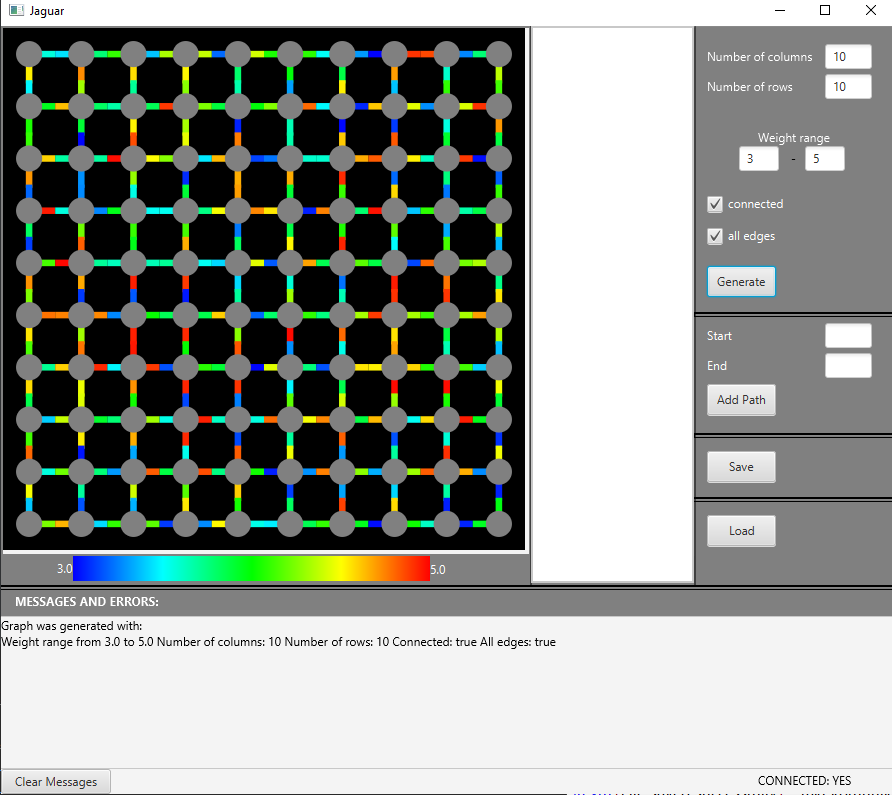
\includegraphics[scale=0.5]{jaguargui.png}
\begin{center}
\texttt{(Rysunek 1)}
\end{center}

Po wybraniu myszką dwóch dowolnych wierzchołków, bądź też wpisaniu ich numerów do zakładki \texttt{Add Path} program powinien wyświetlić nam najkrótszą ścieżkę pomiędzy tymi punktami, wyświetlić okienko z tą ściężką w specjalnym miejscu pomiędzy wizualizacją grafu a trybami generacji (Rysunek 2).

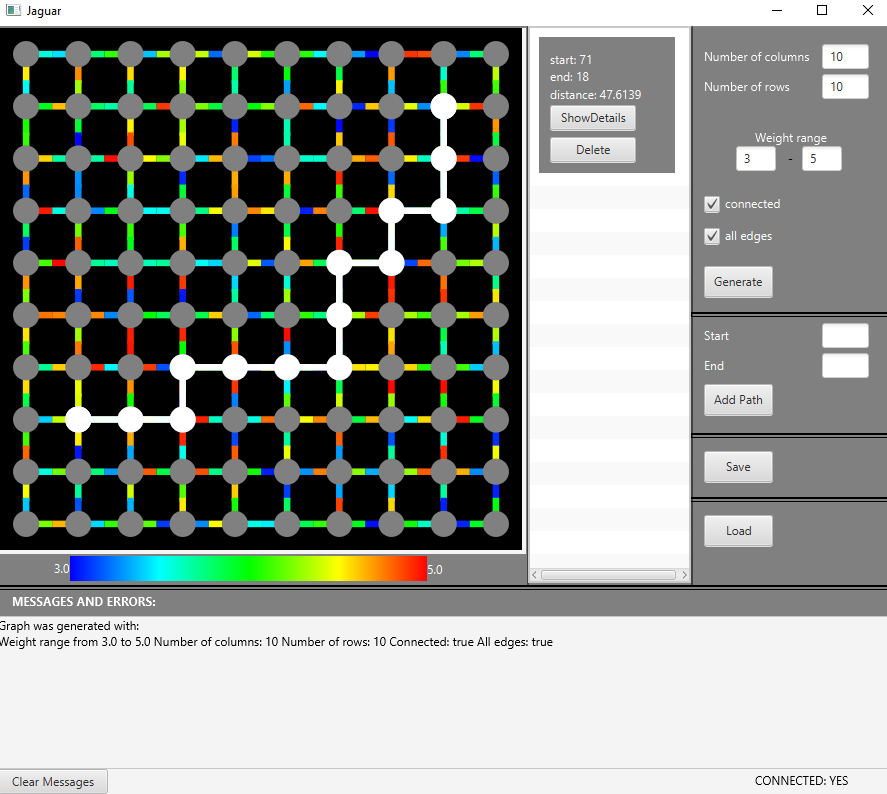
\includegraphics[scale=0.5]{gui_paths}
\begin{center}
\texttt{(Rysunek 2)}
\end{center}

\section{Komunikaty błędów i wiadomości do użytkownika}\label{header-n279}
Komunikaty błędów i wiadomości do użytkowniak zostały zmienione i podawane są w języku angielskim w zakładce \texttt{MESSAGES AND ERRORS}:
\begin{itemize}
\item
\texttt{Number of columns and rows must be integers greater than 1} - taki komunikat dostaniemy, gdy podamy liczbę wierszy lub kolumn do wygenerowania mniejszą bądź równą 1;
\item
\texttt{Weight range must be real number greater than 0 and number of columns and rows must be integers greater than 1} - taki komunikat otrzymamy, gdy wpiszamy dane w złym formacie. Przykładowo gdy podamy zakres wag jako ww-ee lub gdy wpisana liczba będzie zbyt duża;
\item
\texttt{Min and max must be real number greater than 0} - taki komunikat otrzymamy, gdy podamy wartość wag mniejszą niż 0;
\item
\texttt{File saved successfully} - taki komunikat otrzymamy, gdy zapiszemy plik we wskazanej lokalizacji;
\item
\texttt{File was loaded successfully} - taki komunikat otrzymamy, gdy uda nam się pomyślnie wczytać plik;
\item
\texttt{Couldn't load the file} - taki komunikat otrzymamy, gdy nie uda nam się wczytać wskazanego pliku;
\item
\texttt{Graph was generated with:}

\texttt{Weight range from x to y Number of columns: z Number of rows: w Connected: true/false All edges: true/false}
 - taki komunikat dostaniemy po wygenerowaniu grafu z liczbą kolumn równą z, liczbą wierszy równą w, zakresem wag od x do y oraz dostaniemy informację o tym, czy chcieliśmy wygenerować spójny i czy ze wszystkimi krawędziami.


\end{itemize}

\section{Wnioski}\label{header-n279}
Podczas wykonywania tego projektu mieliśmy styczność z różnymi oprogramowaniami służącymi do pisania kodu. Niewątpliwie najciekawszym z nich był pakiet JavaFX do tworzenia interfejsu graficznego użytkownika. Było to swego rodzaju nowością, jak i wyzwaniem, w porównaniu do poprzedniego projektu, gdzie program działał jedynie w trybie wsadowym. Napisanie algorytmów na podstawie, których działa program nie było już wyzwaniem, gdyż dokładnie tych samych używaliśmy w poprzednim projekcie. Pisząc kod w języku \texttt{Java} mieliśmy również styczność z podejściem obiektowym, które daje ogromne możliwości i znacząco ułatwia pisanie kodu. Współpraca nie przebiegała zbyt łatwo ze względu na to, że przy pisaniu klas dana osoba nie znała wszystkich metod, które potrzebne były drugiej osobie. Skutkowało to koniecznością wprowadzania zmian w klasach oraz dopisywania metod do nich. Dodatkową trudność sprawił fakt, że tak naprawdę dopiero poznawaliśmy ten język, co skutkowało tym, że nie daliśmy rady zastosować wielu rzeczy, które oferuje, a które byśmy przy ponownym pisaniu tego kodu wykorzystali.


\end{document}
